\chapter{Experiments and Evaluation}\label{experiment}

\section{Simulation of Flocking Models}

We first show the influence of $\sigma$ and $\beta$ in (\ref{eq:proposed_ui}) to the convergence of the flock by Fig.\ref{fig:sigma_beta}, where the averaged $\psi_{scal}$ (\ref{eq:psi_scal}) of ten simulation results are illustrated with three cases. The more $\psi_{scal}$ gets close to 1, the more convergent and aligned the flock is. As shown in the figure that the choice of $\sigma$ has little impact on the convergence rate compared with $\beta$. When $\beta\leq\frac{1}{2}$, the convergence of the whole flock is unconditional which is coincident with our assumption in Ch.~\ref{control_law}. Without explicit statement, all the following simulations use $\sigma=1$ and $\beta=0.25$.

\begin{figure}[htb]
  \centering
  \subfigure[Case 1: $\sigma<1$ with $\sigma=0.5$]{\label{fig:sigma0_5}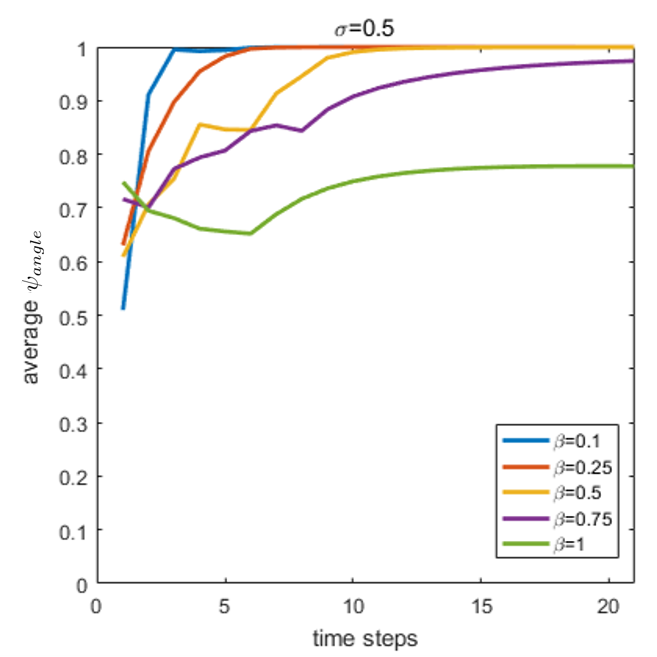
\includegraphics[width=0.48\textwidth]{figure/chapter_5/sigma0_5.png}}
  \subfigure[Case 2: $\sigma=1$]{\label{fig:sigma1}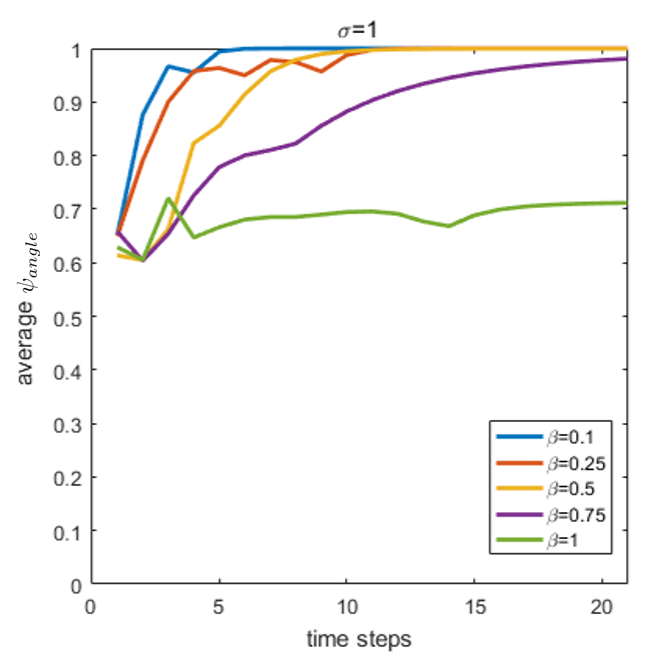
\includegraphics[width=0.48\textwidth]{figure/chapter_5/sigma1.png}}
  \quad
  \subfigure[Case 3: $\sigma>1$ with $\sigma=1.5$]{\label{fig:sigma1_5}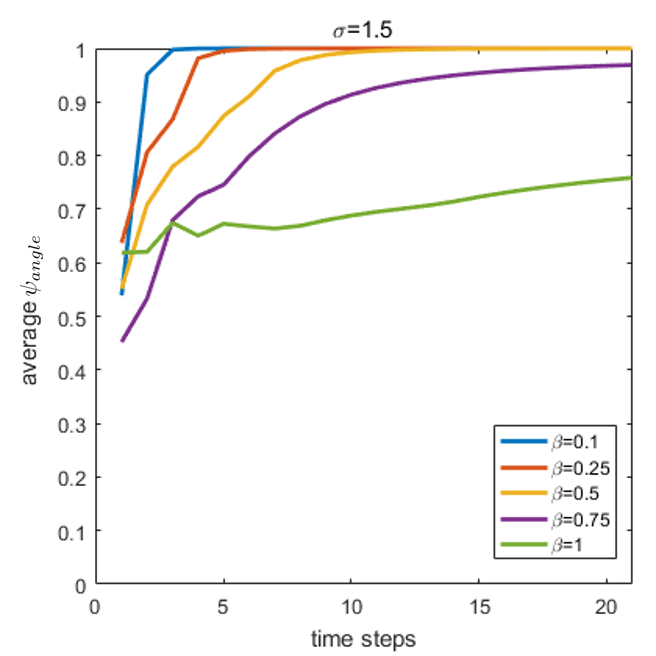
\includegraphics[width=0.48\textwidth]{figure/chapter_5/sigma1_5.png}}
  \caption{Averaged $\psi_{scal}$ of twenty simulations of two agents w.r.t various $\sigma, \beta$. The initial velocity are all randomized and nonzero.}\label{fig:sigma_beta}
\end{figure}

\begin{figure}[htb]
  \centering
  \subfigure[Multiple agents with fixed $\sigma, \beta$]{\label{fig:multiple}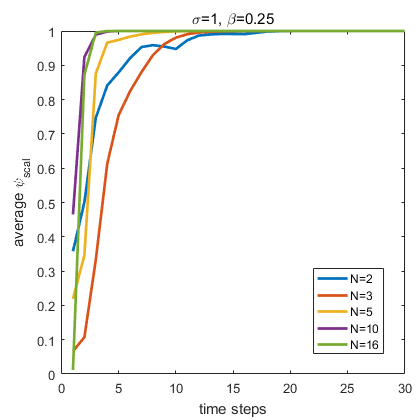
\includegraphics[width=0.48\textwidth]{figure/chapter_5/multiple.png}}
  \subfigure[Multiple agents with fixed $\sigma, \beta$]{\label{fig:distance}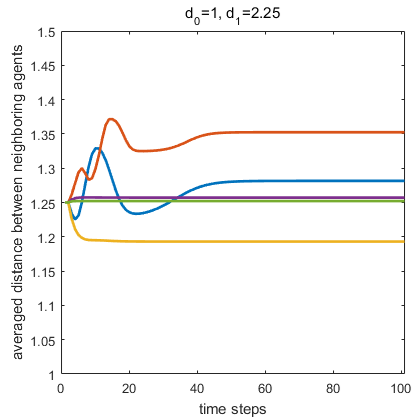
\includegraphics[width=0.48\textwidth]{figure/chapter_5/distance.png}}
  \caption{(a): Fixed $\sigma, \beta$ with various number of agents. The initial velocity are all randomized and nonzero. (b): Corresponding averaged distance between neighboring agents.}\label{fig:multiple_distance}
\end{figure}

We compare our proposed flocking model with the ones in~\cite{Vicsek1995,CuckerSmale2007,CuckerDong2010} in Ch.~\ref{flocking} with 2, 3 and 4 agents respectively. The initial position are illustrated in Fig.\ref{fig:simulate_flocking} where the initial velocities are randomized.
\begin{figure}[htb]
  \centering
  \subfigure[Two agents in a shape of straight line]{\label{fig:2_agents}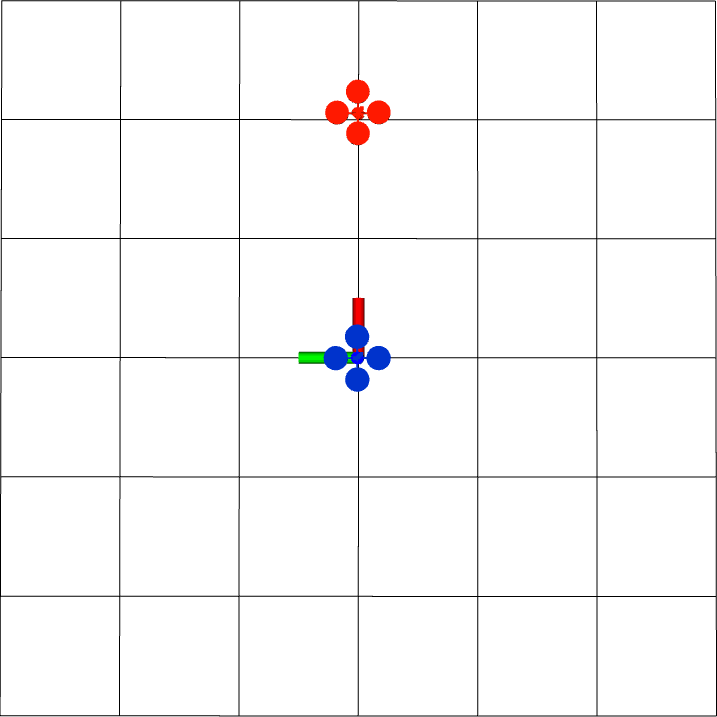
\includegraphics[width=0.32\textwidth]{figure/chapter_5/2_agent.png}}
  \subfigure[Three agents in a shape of equilateral triangle]{\label{fig:2_agents}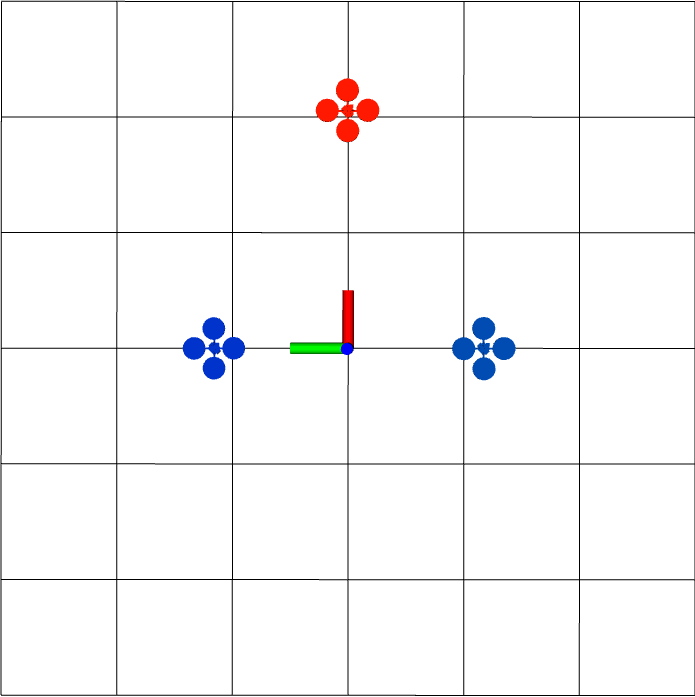
\includegraphics[width=0.32\textwidth]{figure/chapter_5/3_agent.png}}
  \subfigure[Four agents in a shape of diamond]{\label{fig:2_agents}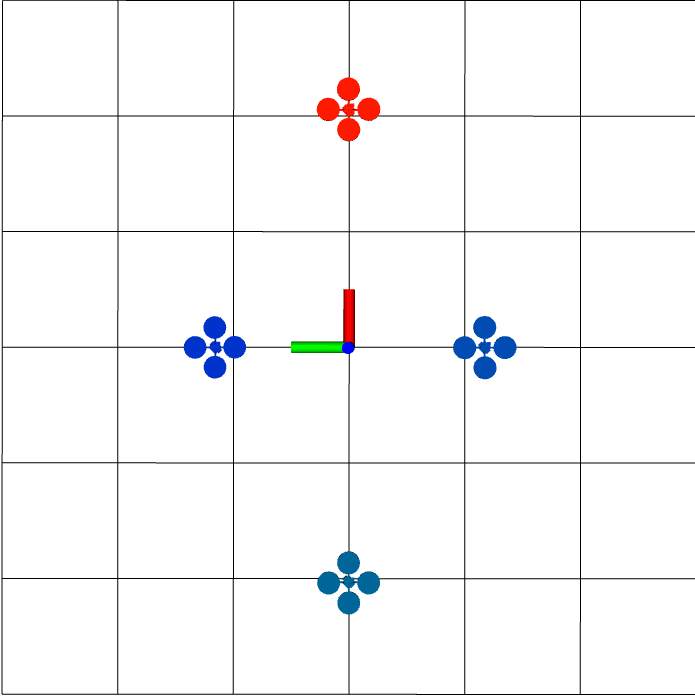
\includegraphics[width=0.32\textwidth]{figure/chapter_5/4_agent.png}}
  \caption{Simulations of multi-UAV flocking}\label{fig:simulate_flocking}
\end{figure}

\begin{figure}[htb]
  \centering
  \subfigure[Multiple agents with fixed $\sigma, \beta$]{\label{fig:N2_scal}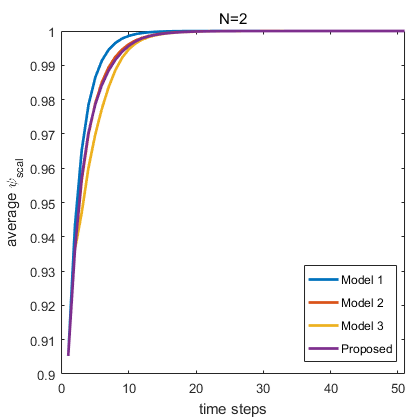
\includegraphics[width=0.48\textwidth]{figure/chapter_5/N2_scal.png}}
  \subfigure[Multiple agents with fixed $\sigma, \beta$]{\label{fig:N3_scal}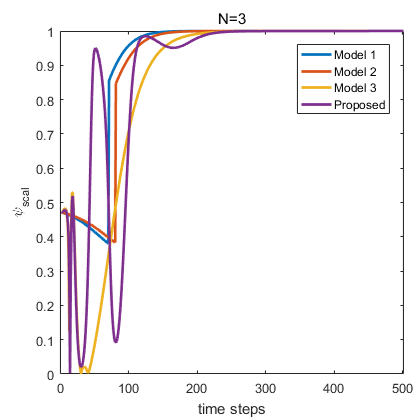
\includegraphics[width=0.48\textwidth]{figure/chapter_5/N3_scal.png}}
  \quad
  \subfigure[Multiple agents with fixed $\sigma, \beta$]{\label{fig:N4_scal}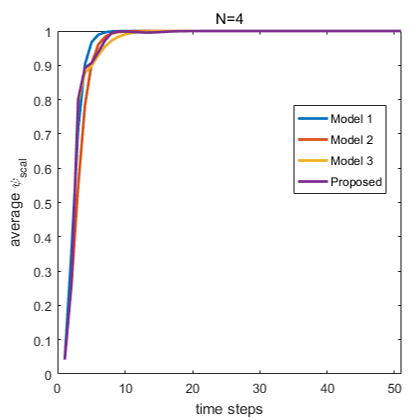
\includegraphics[width=0.48\textwidth]{figure/chapter_5/N4_scal.png}}
  \caption{TODO}\label{fig:N_scal}
\end{figure}

\begin{figure}[htb]
  \centering
  \subfigure[Multiple agents with fixed $\sigma, \beta$]{\label{fig:N2_dis}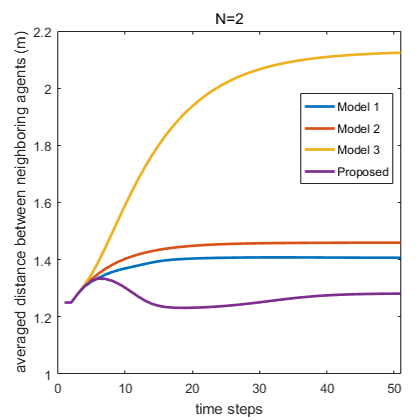
\includegraphics[width=0.48\textwidth]{figure/chapter_5/N2_dis.png}}
  \subfigure[Multiple agents with fixed $\sigma, \beta$]{\label{fig:N3_dis}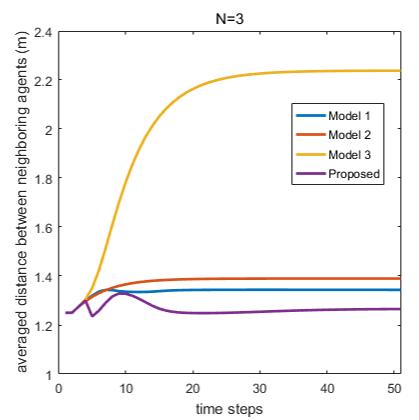
\includegraphics[width=0.48\textwidth]{figure/chapter_5/N3_dis.png}}
  \quad
  \subfigure[Multiple agents with fixed $\sigma, \beta$]{\label{fig:N4_dis}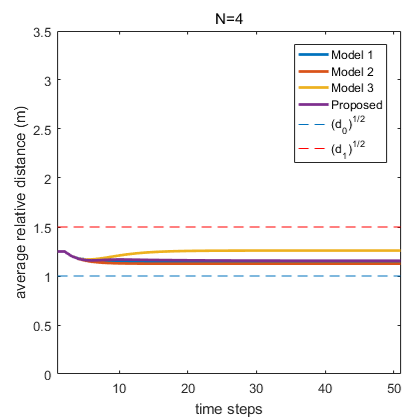
\includegraphics[width=0.48\textwidth]{figure/chapter_5/N4_dis.png}}
  \caption{TODO}\label{fig:N_dis}
\end{figure}

\section{Comparison with Tracking Problem}

We have compared the cohesion, separation and alignment performance from our proposed flocking model with those solved by traditional tracking algorithm inspired by~\cite{Chenjing}. As shown in~\ref{fig:rviz}

\begin{figure}[htb]
  \centering
  \subfigure[TODO]{\label{fig:rviz}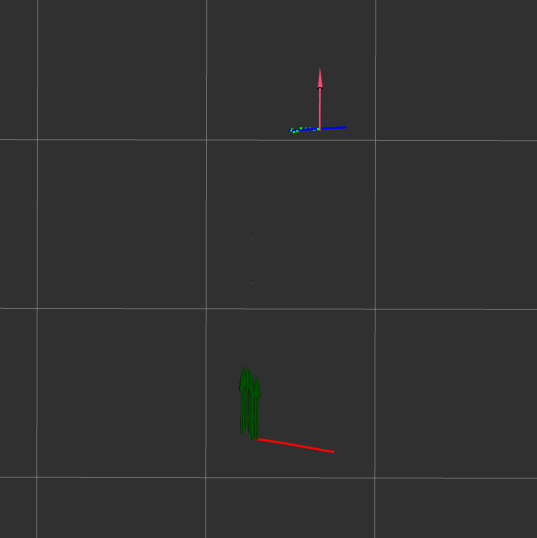
\includegraphics[width=0.48\textwidth]{figure/chapter_5/predict_plan.png}}
  \subfigure[TODO]{\label{fig:capture}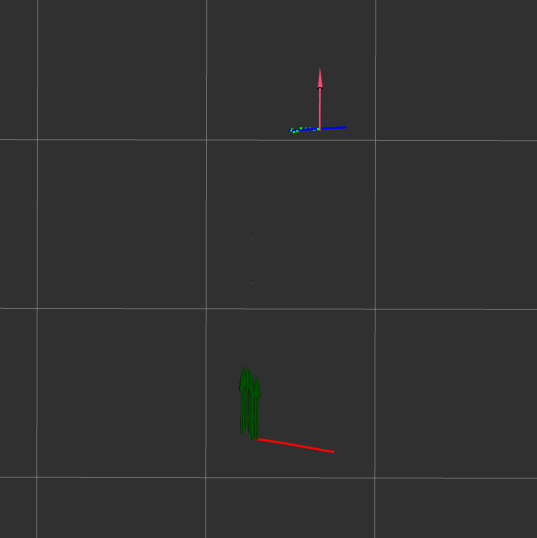
\includegraphics[width=0.48\textwidth]{figure/chapter_5/predict_plan.png}}
  \caption{Screenshots of rviz and camera. Left: Target motion prediction and trajectory planning.}\label{fig:rviz_capture}
\end{figure}

\subsection{Target Motion Estimation and Prediction}

We denote the 3D position of the target at time t $\in \mathbb{R}$ as T(t) $\in \mathbb{R}^{3}$ and expand it with Taylor Series. We omit the high order terms $(n>5)$ and approximate it with the $5^{th}$ order polynomial $\hat{T}(t) \in \mathbb{R}^{3}$:
\begin{equation}\label{eq:poly5}
T(t) = \sum^n_{i=0} a_{i}t^i
\approx \sum^5_{i=0} a_{i}t^i
= \begin{bmatrix}1\\t\\t^2\\t^3\\t^4\\t^5\end{bmatrix}^T\begin{bmatrix}a_0\\a_1\\a_2\\a_3\\a_4\\a_5\end{bmatrix}
= T^TA = \hat{T}(t)
\end{equation}
\noindent
Assuming the target's motion is smooth and continuous, we add acceleration regulator $\lambda_{t}$ and minimize the following:
\begin{equation}\label{eq:minT}
\min_{\hat{T}(\cdot)} \sum^{L}_{i=0} ||\hat{T}(t_i)-p_i||^2_2 + \lambda_t\int_{t_l}^{t_m} ||\hat{T}^{(2)}(t)||^2_2dt
\end{equation}
\noindent
where $L$ is the total number of observations captured and $p_i$ is the $i^{th}$ target position in global frame at time $t_i$. Note here that $[t_l, t_0]$ is the time period we actually have target observations and $[t_0, t_m]$ is the period we make predictions for target's motion (\ref{eq:minF}).


\subsection{Trajectory Generation}

During the tracking task, the chaser UAV is expected to keep a fixed distance $d_s\in\mathbb{R}^{3}$ from the target. In this scenario, the chaser UAV is supposed to follow the shifted predicted target trajectory $T_s(t)=\hat{T}(t)+d_s$. Similarly, we denote the planned trajectory for chaser UAV with $f(t)=\sum^5_{i=0} e_{i}t^i=T^TE$ and adjust the tracking stiffness with regulator $\lambda_f$. We then minimize the following:

\begin{equation}\label{eq:minF}
\min_{f(\cdot)} \int_{t_0}^{t_m} ||f(t)-T_s(t)||^2_{2}dt + \lambda_f\int_{t_0}^{t_m} ||f^{(3)}(t)||^2_{2}dt
\end{equation}
\indent s.t.
\begin{equation}
\underbrace{f(t_0)=f_0}_{\text{initial state constraint}}
\end{equation}
\begin{equation}
\underbrace{f(t_m)=0}_{\text{ending state constraint}}
\end{equation}
\begin{equation}
\underbrace{f^{(1)}(t) \in \Omega_{v}(t)}_{\text{velocity constraint}}
\end{equation}
\begin{equation}
\underbrace{f^{(2)}(t) \in \Omega_{a}(t)}_{\text{acceleration constraint}}
\end{equation}
\noindent
where $f_0$ is the state of the chaser UAV at the beginning of the trajectory and $\Omega_v$ and $\Omega_a$ are the velocity and acceleration constraints respectively.

We can rewrite (\ref{eq:minF}) as:
\begin{equation}\label{eq:reminF1}
\min_{l\in\{x,y,z\}}\int_{0}^{t_m-t_0} (A^TT_sT_s^TA-2E^TT^TT_s^TA+E^TT^TTE)dt + \lambda_f\int_{0}^{t_m-t_0} (E^TT_fT_f^TE)dt\\
\end{equation}
\noindent
and transform (\ref{eq:reminF1}) into a standard QP problem:
\begin{equation}\label{eq:reminF2}
\min_{l\in\{x,y,z\}}E^T[\int_{0}^{t_m-t_0}(T^TT+T_fT_f^T)dt]E-2E^T[\int_{0}^{t_m-t_0}T_f^TT_s^T]A
\end{equation}
\noindent
where $T_s = \begin{bmatrix}1\\1+dT\\(1+dT)^2\\(1+dT)^3\\(1+dT)^4\\(1+dT)^5\end{bmatrix}$ and $T_f=\begin{bmatrix}0\\0\\0\\6\\24t\\60t^2\end{bmatrix}$ with $dT=t_0-t_l$. We use $l\in\{x,y,z\}$ to abstract the dimension.

\subsection{Performance Comparison}



\newpage